\chapter{Firewall Testing}
	\label{firewalltesting}

	
	\begin{landscape}
	\section{Testgeräte}
	\begin{tabularx}{1.4\textwidth}{|l|XXX|}
		\hline
		\textbf{Abbildung} & \textbf{Gerät} & \textbf{Hardware} & \textbf{Software}\\
		\hline
		
\includegraphics[width=3cm]{../performanceAnalaysis/devices/asusux21.png} & Ultrabook, Asus UX 31 & Intel Core i7 2x 1.8 GHz, 3.8GiB Memory
& Ubuntu 12.04 64Bit, Browser: Firefox 25 \\
		\hline
		
\includegraphics[width=3cm]{../performanceAnalaysis/devices/samsungnc10.jpg} & Netbook, Samsung NC 10 & Intel Atom 1.6 GHz, 992MiB Memory & Ubuntu 12.10 32Bit, Browser: Firefox 23 \\
		\hline
		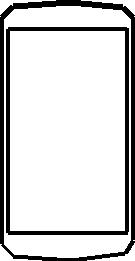
\includegraphics[width=3cm]{../performanceAnalaysis/devices/googlenexus4.jpg} & Smartphone, Google Nexus 4 & NQualcomm Snapdragon S4 Pro 2x 1.5 GHz, 2GB Memory & Android 4.3 32 Bit, Firefox 25 \\
		\hline
	\end{tabularx}
	
	
	\section{Testszenarien und Ergebnisse}
	
		\subsection{VPN-Locale}
			\begin{tabularx}{1.4\textwidth}{|lXX|}
				\hline
				\textbf{Geräte} & \textbf{Setup} & \textbf{Ergebnisse} \\
				\hline
					Home-WLAN - Home-WLAN-HSR-VPN
				&
					• Smartphone über lokales Home-WLAN, Cablecom 10er-Leitung\newline
					• Ultrabook über lokales Home-WLAN, Cablecom 10er-Leitung,
					Verbunden mit HSR-VPN\newline
				& 
					• Media-Stream kommt ohne Verzögerung zustande\newline
					• Kein Unterschied zu Locale Round\\
				\hline
			\end{tabularx}
	
		\subsection{HSR-Mobile}
			\begin{tabularx}{1.4\textwidth}{|lXX|}
				\hline
				\textbf{Geräte} & \textbf{Setup} & \textbf{Ergebnisse} \\
				\hline
					Mobile-Network - HSR-Notebook-WLAN
				&
					• Netbook über Mobilfunk, Sunrise Mobile Prepaid (max. 256 Kbps)\newline
					• Ultrabook über HSR-Notebook-WLAN\newline
				& 
					• Media-Stream kommt nicht zustande\newline
					• Im Wireshark sind keine UDP-Pakete sichtbar\newline
					• Vermutung: HSR blockt ``dynamic port''-``dynamic port''-Verbindungen um
					Filesharing zu unterbinden\newline
					• Auch die apprtc.appspot.com-Demo-App kommt nicht durch\\
				\hline
			\end{tabularx}
				
	\end{landscape}
